\documentclass[superscriptaddress, amsmath,preprintnumbers,10pt,article,notitlepage]{revtex4-1}
%\documentclass[superscriptaddress, twocolumn, prl, longbibliography, nofootinbib]{revtex4-1}
\usepackage{amsmath}
\usepackage{amsbsy}
\usepackage{amssymb}
\usepackage{graphicx}
\usepackage{color}
\usepackage{subfigure}
\usepackage{physics}
\usepackage{soul}
\usepackage{color}
\usepackage{bm}
\usepackage{array}
\usepackage{multirow}
\usepackage{lipsum}
\usepackage[normalem]{ulem}
%\newcommand{\Tr}{\text{Tr}}
\newcommand{\Ai}{\text{Ai}}
\newcommand{\Bi}{\text{Bi}}
\newcommand{\Real}{\text{Re}}
\newcommand{\Imag}{\text{Im}}
\newcommand{\T}{T}
\newcommand{\U}{U}
\usepackage{verbatim}
\usepackage{natbib}

\usepackage[pdftex,colorlinks=true,
	pdfstartview = FitV,
	linkcolor    = linkcolor,
	citecolor    = linkcolor,
	urlcolor     = linkcolor,	
	hyperindex   = true,
	hyperfigures = false]{hyperref}

\newcommand{\ee}{\text{e}}
\newcommand{\A}{\text{\tiny{A}}}

\DeclareMathOperator\erf{erf}
\newcommand\mymathop[1]{\mathop{\operatorname{#1}}}

\def\smath#1{\text{\scalebox{0.9}{$#1$}}}
\def\sfrac#1#2{\smath{\frac{#1}{#2}}}


\bibliographystyle{apsrev4-1}
\begin{document}

\title{Supplementary information: Inferring dissipation from static structure in active matter}

\author{Laura Tociu}
\author{Gregory Rassolov}
\affiliation{James Franck Institute, University of Chicago, Chicago, IL 60637}
\affiliation{Department of Chemistry, University of Chicago, Chicago, IL 60637}

\author{\'Etienne Fodor}
\affiliation{Department of Physics and Materials Science, University of Luxembourg, L-1511 Luxembourg}

\author{Suriyanarayanan Vaikuntanathan}
\affiliation{James Franck Institute, University of Chicago, Chicago, IL 60637}
\affiliation{Department of Chemistry, University of Chicago, Chicago, IL 60637}

\maketitle

\section{Derivation of Pair Correlation Function and Rate of Work}
We begin with Eq.~(3) in the main text, and we do not consider the polarization term further. Our choice is justified in the low-activity limit and, beyond that, supported by the results in~\cite{Suri2020} in main text. In this work, the formulas for efficiency and mobility were obtained by setting two-point polarization correlators to zero, see Eqs.~(A.8-A.9) in Appendix A, and the results agree with simulation data very well even at strong driving. Ignoring polarization results in a closed-form equation of motion for the field that can be linearized around the density $\rho_0$ of the particles by writing $\rho ({\bf r}, t) = \rho_0 + \delta \rho({\bf r}, t)$ and discarding the terms quadratic in $\delta \rho$. This approximation holds for weak interparticle potentials so that any local density fluctuation is small compared to the density of the liquid. 

After linerization, the solution for $\delta \rho({\bf k}, t) = \int [ \rho({\bf r}, t) - \rho_0 ] e^{-i{\bf k} \cdot {\bf r}} d{\bf r}$ follows readily as:

\begin{equation}\label{eq:red_field_EOM_k}
\delta \rho( {\bf k}, t)  = \int_{-\infty}^t e^{-|{\bf k}|^2 G({\bf k}) (t-s)} \left( -h |{\bf k}|^2 \rho_0 \U({\bf k}) e^{-i{\bf k} \cdot {\bf r}_0(t - s)} + i{\bf k} \cdot \sqrt{2\rho_0 \T} \bm{\Lambda} ({\bf k}, s) \right) ,
\end{equation}
where $G({\bf k}) =  T + \rho_0U({\bf k})$, and 
\begin{equation}\label{eq:field_noise_k}
\langle \Lambda_{\alpha}({\bf k}, s)  \Lambda_{\beta}({\bf k}', s')  \rangle = (2\pi)^d \delta_{\alpha \beta}\delta(s-s')\delta({\bf k} + {\bf k}') ,
\end{equation}
where $d$ is the spatial dimension.


\subsection{Derivation of Rate of Work}

Substituting the field Eq. \ref{eq:red_field_EOM_k} into
\begin{align}\label{eq:wdot}
    \dot{w} & = \sum_{i, j\neq i} \big\langle {\bf f}_i \cdot \nabla_i U({\bf r}_i-{\bf r}_j) \big\rangle \nonumber \\
    & = h \int \big\langle {\bf f}_i(t) \cdot i{\bf k} \U({\bf k}) \,\delta \rho({\bf k}, t) \big\rangle \,d{\bf k} 
\end{align}
gives:

\begin{align}
\dot{w} & =  -h^2\dfrac{\rho_0}{\gamma} \int d{\bf k} |{\bf k}|^2 (U({\bf k}))^2  \int
_{-\infty}^0 ds e^{|{\bf k}|^2 G({\bf k})s} \langle i{\bf k} \cdot {\bf f}_0(0) e^{i{\bf k}\cdot ({\bf r}_0(0) - {\bf r}_0(s))}\rangle + \nonumber \\
& h\dfrac{1}{\gamma} \int d{\bf k} |{\bf k}|^2 U({\bf k})  \int
_{-\infty}^0 ds e^{|{\bf k}|^2 G({\bf k})s} \left \langle e^{i{\bf k}\cdot {\bf r}_0(0)} {\bf f}_0(0) \cdot  {\bm \Lambda}({\bf k}, s)\right \rangle 
\end{align}
Truncating at second order in parameter $h$, we get:
\begin{align}
\dot{w} & =  -h^2\dfrac{\rho_0}{\gamma}   \int d{\bf k} |{\bf k}|^2 (U({\bf k}))^2 \int_{\infty}^0 ds e^{|{\bf k}|^2 G({\bf k})s}  \langle i{\bf k} \cdot {\bf f}_0(0)   e^{i{\bf k}\cdot \int_s^0 [1/\gamma {\bf f}_0(x) + {\bm \xi}_0(x)] dx}  \rangle - \nonumber \\
&  h^2 \dfrac{\rho_0}{\gamma}  \int d{\bf k} \int d{\bf k}' |{\bf k}|^2 |{\bf k}'|^2 U({\bf k}) U({\bf k}') \int_{-\infty}^0 ds' e^{- |{\bf k}'|^2 G({\bf k}') s'}  \langle  i{\bf k} \cdot {\bf f}_0(0) e^{i{\bf k}\cdot \int_{-\infty}^0 [1/\gamma {\bf f}_0(x) + {\bm \xi}_0(x) ]dx}  e^{i{\bf k}'\cdot \int_{-\infty}^{s'} [1/\gamma {\bf f}_0(x) + {\bm \xi}_0(x)] dx}    \rangle \nonumber \\
& \int_{-\infty}^{0} ds  \int_{-\infty}^{s'} ds'' e^{ |{\bf k}'|^2 G({\bf k}) (s''+s)}  \langle {\bm \Lambda}({\bf k}, s) \cdot {\bm \Lambda({\bf k}', s'')}\rangle
\end{align}


According to Wick's theorem, we can now write for the white noise:

\begin{equation}\label{eq:expxi}
\left \langle e^{i{\bf k}\cdot \int_{s}^0 {\bm \xi}_0(x) dx} \right\rangle =e^{-\frac{|{\bf k}|^2}{\gamma^2} T} 
\end{equation}

Starting from the time correlations of the active forces:

\begin{equation*}\label{eq:active_corr}
\langle f_{i\alpha}(t) f_{j\beta}(0) \rangle = \frac{T_{A}}{\tau} \delta_{ij} \delta_{\alpha\beta} e^{-|t|/\tau},
\end{equation*}
we can derive the following:
\begin{equation*}
\left \langle \int_{s}^0 f_{0\alpha}(0) f_{0\alpha} (x) dx \right \rangle = T_\A (1 - e^{-s/\tau})
\end{equation*}
and
\begin{equation*}
 \left \langle \int_{s}^0 \int_{s}^0  f_{0\alpha} (x)  f_{0\alpha} (x')  dx dx' \right \rangle  =  \int_{s}^0 \int_{x}^0 e^{-(x'-x)/\tau} dx' dx +  \int_{s}^0 \int_{s}^x e^{-(x-x')/\tau} dx' dx = 2T_\A s - 2 T_\A \tau (1 - e^{-s/\tau}) 
\end{equation*}
We will call the above $R(s)$:
\begin{equation*}
R(s) = 2T_\A s - 2 T_\A \tau (1 - e^{-s/\tau}) 
\end{equation*}

According to Wick's theorem, we can now write:

\begin{equation}\label{eq:expf}
\left \langle e^{i{\bf k}\cdot \int_{s}^0 1/\gamma{\bf f}_0(x) dx} \right\rangle =e^{-\frac{|{\bf k}|^2}{\gamma^2} R(-s)/2} 
\end{equation}

This enables us to evaluate the form that we need:

\begin{align}\label{eq:f_time_expf}
\left \langle i{\bf k} \cdot {\bf f}_0(0) e^{i{\bf k} \int_s^0 1/\gamma {\bf f}_0(x) dx} \right \rangle &  = -\dfrac{|{\bf k}|^2}{\gamma} \left \langle  \int_s^0 f_{0\alpha}(0) \cdot f_{0\alpha}(x) dx \right \rangle e^{-\frac{|{\bf k}|^2}{\gamma^2}R(-s)/2} \nonumber \\
& = -\dfrac{|{\bf k}|^2}{\gamma} e^{-\frac{|{\bf k}|^2}{\gamma^2}R(-s)/2} T_\A (1-e^{s/\tau}) 
\end{align}


Going back to the expression for the rate of rate, we can collapse the delta functions in ${\bf k} + {\bf k}'$ and $s-s''$ and use Eq. (\ref{eq:expxi}, \ref{eq:f_time_expf} ),  we get:

\begin{align*}
\dot{w} & = h^2 \rho_0 \dfrac{T_\A}{\gamma^2} \int d{\bf k} |{\bf k}|^4 (U({\bf k}))^2  \Bigl[ \int
_{-\infty}^0 ds e^{|{\bf k}|^2 ( G({\bf k}) + T/ \gamma)s}  e^{-\frac{|{\bf k}|^2}{\gamma^2} R(-s)/2} (1-e^{s/\tau})  + \\
&  \dfrac{T}{\gamma G({\bf k})} \int_{-\infty}^0 ds'  e^{|{\bf k}|^2 ( G({\bf k}) + T/ \gamma)s'}  e^{-\frac{|{\bf k}|^2}{\gamma^2} R(-s')/2} (1-e^{s'/\tau}),
\end{align*}

Therefore, the general formula for rate of work is 

\begin{equation}\label{eq:final_expression_wdot}
\dot{w}  =  \rho_0 \dfrac{T_\A}{\gamma^2} \int d{\bf k} |{\bf k}|^4 (h U({\bf k}))^2 \dfrac{ G({\bf k}) + T/ \gamma}{G({\bf k})}
\int_{-\infty}^0 ds e^{|{\bf k}|^2 ( G({\bf k}) + T/ \gamma)s}  e^{-\frac{|{\bf k}|^2}{\gamma^2} R(-s)/2} (1-e^{s/\tau})
\end{equation}


\subsection{Pair Correlation function}

We substitute  the field Eq.~\eqref{eq:red_field_EOM_k} into
\begin{align*}
\rho_0 g({\bf k}) & = \int d{\bf r} e^{i{\bf k} \cdot{\bf r}} \left \langle  \delta \rho( {\bf r}_0 + {\bf r} ) \right \rangle \\ 
& =  \int d{\bf r} e^{-i{\bf k} \cdot{\bf r}} \left \langle   \int d{\bf k}' e^{i{\bf k}' \cdot( {\bf r} +  {\bf r}_0) } \bar{\rho}({\bf k}') \right \rangle \\ 
& =  \left \langle  e^{i{\bf k} \cdot {\bf r}_0 } \delta \rho({\bf k}) \right \rangle. 
\end{align*}

To at most second order in $h^2$, we get:
\begin{align*}
\rho^2_0 g({\bf k}) & =  \rho_0 \left \langle e^{i{\bf k} \cdot {\bf r}_0(0) }  \int_{-\infty}^0 ds e^{|{\bf k}|^2 G({\bf k})s}  \left[ -h \rho_0 |{\bf k}|^2 U({\bf k}) e^{-i{\bf k} \cdot {\bf r}_0(s)} + i{\bf k}\cdot  {\bm \Lambda}({\bf k}, s) \right] \right \rangle \\
& = - h \rho_0 |{\bf k}|^2 \rho_0  U({\bf k}) \int
_{-\infty}^0 ds e^{|{\bf k}|^2 ( G({\bf k}) + T/ \gamma)s}  e^{-\frac{|{\bf k}|^2}{\gamma^2} R(-s)/2} - \\
&  h \dfrac{\rho_0}{\gamma}  \int d{\bf k}'  |{\bf k}|^2 |{\bf k}'|^2 U({\bf k}') \int_{-\infty}^0 ds' e^{ |{\bf k}'|^2 G({\bf k}') s'}  \langle e^{i{\bf k}\cdot \int_{-\infty}^0 [1/\gamma {\bf f}_0(x) + {\bm \xi}_0(x) ]dx}  e^{i{\bf k}'\cdot \int_{-\infty}^{s'} [1/\gamma {\bf f}_0(x) + {\bm \xi}_0(x)] dx}    \rangle \\
& \int_{s}^{0} ds  \int_{-\infty}^{s'} ds'' e^{ |{\bf k}'|^2 G({\bf k}) (s''+s)}  \langle {\bm \Lambda}({\bf k}, s) \cdot {\bm \Lambda}({\bf k}', s'')\rangle ,
\end{align*} where $R(s)=2T_\A s - 2T_\A \tau (1- e^{-s/\tau})$.



Collapsing noise correlation functions and using Eq. (\ref{eq:expxi}, \ref{eq:expf}) we obtain that the form of the pair correlation function is:

\begin{equation}\label{eq:final_expression_gr}
\rho^2_0 g({\bf k}) = 
& - \rho_0 ( |{\bf k}|^2 \rho_0 h U({\bf k}))  \dfrac{ G({\bf k}) + T/ \gamma}{G({\bf k})} \int
_{-\infty}^0 ds e^{|{\bf k}|^2 ( G({\bf k}) + T/ \gamma)s}  e^{-\frac{|{\bf k}|^2}{\gamma^2} R(-s)/2}  
\end{equation}



\subsection{Derivation of $\tilde{I}$}
We are interested in the quantity $\tilde{I} = \dot{w} - h^2 \rho_0^2 \int d{\bf k} |{\bf k}|^2 (U({\bf k}))^2 (g - g_{eq})({\bf k})$, up to order $h^2$. This expression can be easily calculated using the expressions for rate of work and  the pair correlation function (setting $T_A =  0$) derived in the previous sections. The result is:

\begin{align}\label{eq:final_expression_I}
\mathcal{I} & =   \rho_0 \int d{\bf k} |{\bf k}|^4 (h U({\bf k}))^2 \dfrac{ G({\bf k}) + T/ \gamma}{G({\bf k})}
\int_{-\infty}^0 ds e^{|{\bf k}|^2 ( G({\bf k}) + T/ \gamma)s}  e^{-\frac{|{\bf k}|^2}{\gamma^2} R(-s)/2} \nonumber\\
& \left[ T_\A/\gamma^2  (1-e^{s/\tau}) - \rho_0 h U({\bf k}) \right] - \nonumber \\
&h^2 \rho_0 \int d{\bf k} |{\bf k}|^4 (U({\bf k}))^2 \dfrac{ G({\bf k}) + T/ \gamma}{G({\bf k})}
\int_{-\infty}^0 ds e^{|{\bf k}|^2 ( G({\bf k}) + T/ \gamma)s} \rho_0 h U({\bf k})
\end{align}

In order to obtain the plots in Fig. 3 of the main text, the substitution $h U({\bf k}) \rightarrow - T c({\bf k})$ is employed in Eq. \ref{eq:final_expression_wdot} and Eq. \ref{eq:final_expression_I}.

\begin{figure}
    \centering
    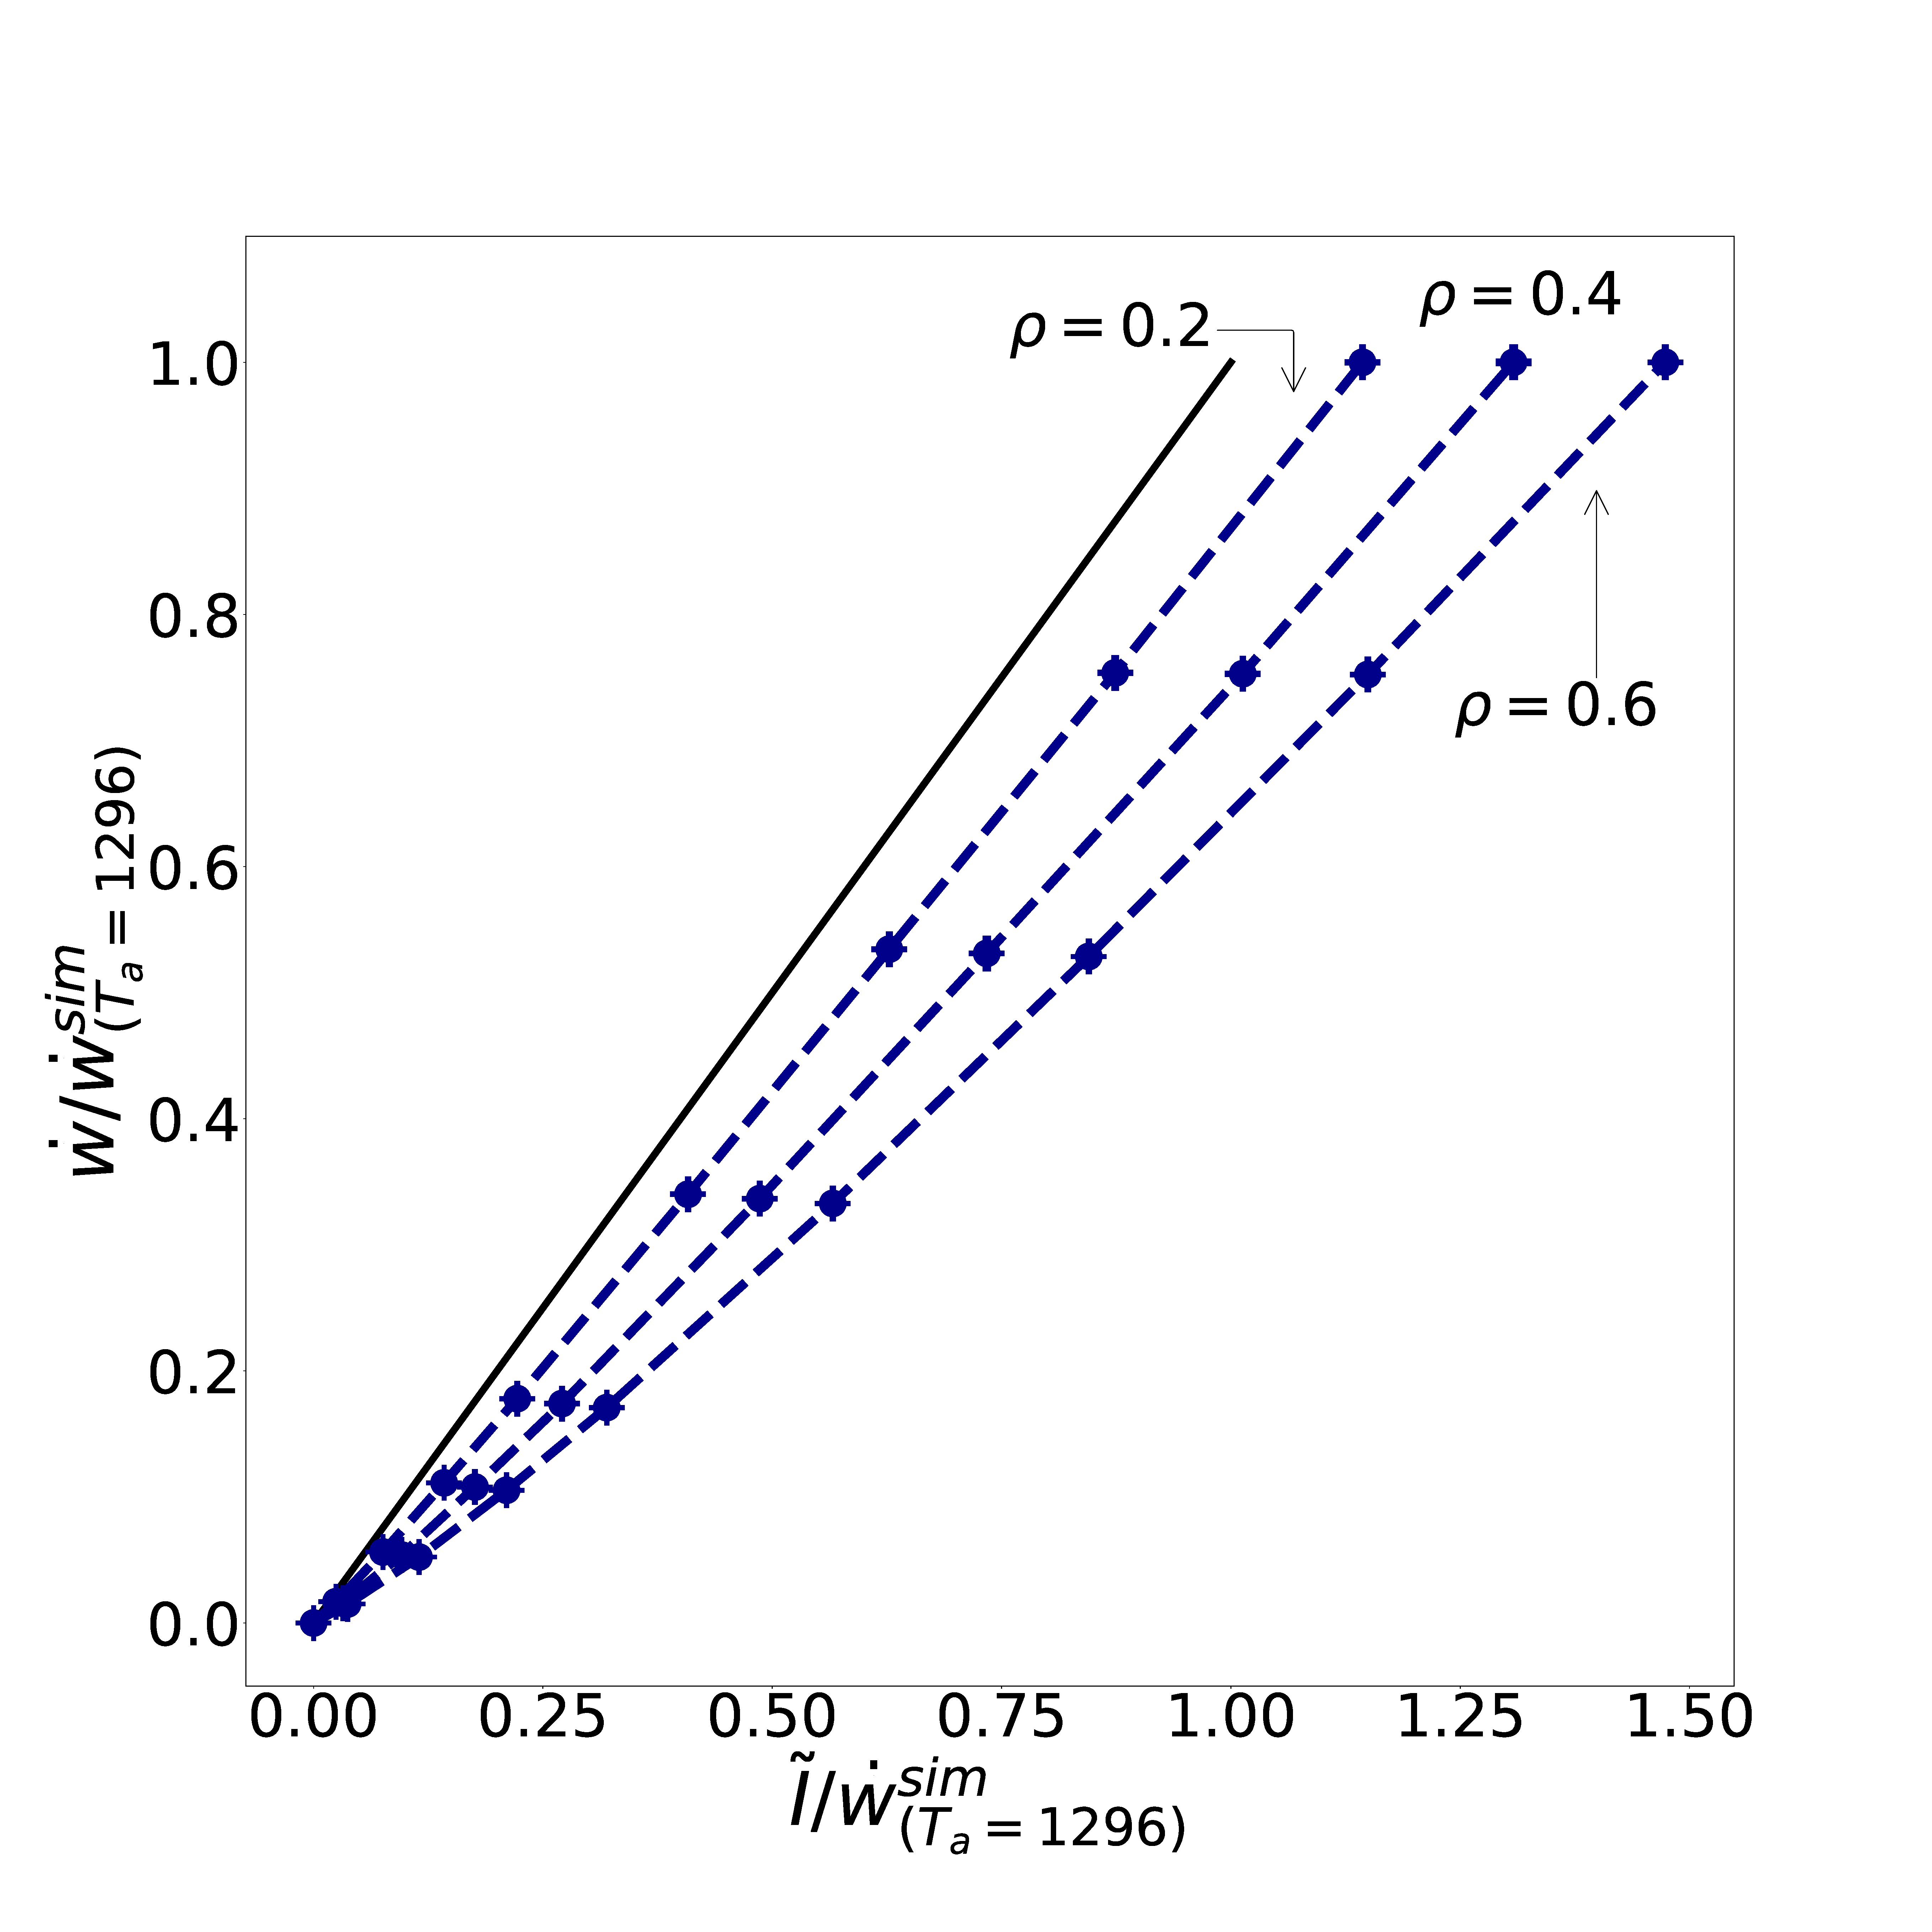
\includegraphics[scale=0.15, clip=True]{Yukawa_Figure.eps}
    \caption{Simulation results for $\dot{w}$ vs $\tilde I$ for particles with the Yukawa interparticle potential (dashed blue lines) at various densities (labeled). While $\dot{w} \neq \tilde I$, the ratio between them is constant essentially constant for values of $T_a$ corresponding ranging from weak to moderately strong driving. Deviation from $\dot{w} = \tilde I$ (solid black line) increases as $\rho$ increases. Parameters: Yukawa potential, $A=50$, $\kappa=4.0$ $\tau=1.0$, $0<=T_a<=1296$}
    \label{Fig:S1}
\end{figure}

\section{Continuous Convolutional Neural Network}

The network was built in keras using the Functional API \cite{keras}. The individual input to the network consists of an array of size $N \cross D$ that contains, for each of the N particles, the distances to its nearest $D$ neighbors. For the simulations with the harmonic potential, $N = 625$ and $D = 20$, while for the simulations with the Yukawa potential, $N = 312$ and $D = 25$. The choice of $D$ was such that distances to around $r = 3$ ($r = 4$ for Yukawa) are mostly captured, but with certainty all distances up to the cutoff ($r = 1$ for harmonic and $r=2.5$ for Yukawa) are captured. Such a choice ensures that the algorithm has access to all the distances that we expect are crucial to extracting the rate of work, but also simplifies the implementation by allowing a rectangular input shape.

The continuous convolutional layer is built as a custom layer and performs the following:
For each convolution center, in this case an AOUP particle ${\bf r}_i$, the convolution operation consists of evaluating the sum $\sum_{j=1}^{D} F({\bf r}_{ij})$. Here, $F$ is a learnable function, the equivalent of a filter in traditional convolutional neural networks.  Inspired by our connection between interparticle distances and rate of work in Section XXX (Eq. YYY), we relax the function $F$ to be a radial function, and we express it in a basis of $N_G=30 $ ( $N_G=40 $  for Yukawa) Gaussian functions centered between $r=0$ and $r=3$ ($r = 4$ for  Yukawa) and with a standard deviation of 0.05:

\begin{equation}
    F(r) = \sum_{i=0}^{15} \beta_i e^{-(r-0.2 i)^2/(2\cdot 0.1)^2}
\end{equation}

In the dense layer, we enforce particle indistinguishibility by setting a constraint that the weights $u_i = u $ are identical. 

Finally, the output to the network consists of the rate of work $\dot{w}$, centered as:

\begin{equation}
    \dot{w}_{\text{centered}} = \dot{w} + \alpha \int 2\pi r (\nabla u(r)^2 - \nabla^2 u(r)) g_{eq}(r) dr
\end{equation}

and rescaled as:

\begin{equation}
    \dot{w}_{\text{rescaled}} = \dfrac{\dot{w}_{\text{centered}}}{\max(\dot{w}_{\text{centered}}) - \min(\dot{w}_{\text{centered}} )}
\end{equation}

The rate of work is calculated at each value of $T_A$ as detailed in the main text. Multiple individual snapshots at the same value of $T_A$ will have the same output.

In conclusion, the machine performs the following mapping from the interparticle distances $r_{ij}$ to the output (rescaled rate of work):

\begin{equation}
     u \sum_i \sum_{j} \sum_{k=0}^{15} \beta_k e^{-(r_{ij}-0.2 i)^2/(2\cdot 0.1)^2} + b = \dot{w}_{\text{rescaled}}
\end{equation}

The machine is tasked with finding the best $u, \beta_k$ and $b$ to minimize the deviation between its predicted output $\dot{w}_{\text{pred}}$ and $\dot{w}_{\text{rescaled}}$. We choose to quantify this deviation through a loss function of the form:

\begin{equation}
     L(\{\dot{w}^a_{pred, i}\}) = \sum_a \left[  \left( \dfrac{\sum_i \dot{w}^a_{pred, i}}{N_a} \right) - \dot{w}^a_{\text{rescaled}} \right]^2,
\end{equation}
where the $a$ indexes the $T_A$ values used in the training process and $N_A$ is the number of snapshots in each training batch over which the loss function is calculated. Our choice of loss function ensures that we are mapping the average of the output of the  network at each $T_\A$ to the rate of work at the same $T_\A$. Since the rate of work is indeed an average function of the configurations, this choice of loss function was the most suitable for training our model.

Acknowledging that in the large $N$ limit, $ \int 2\pi r F(r) g(r) dr = 1/N \sum_i \sum_j F(r_{ij})$, and using Eq. XXX, it follows that the machine learning could, in principle, learn the mapping exactly by setting $b = 0$, $ u = \alpha/(\text{N} (\max(\dot{w}_{\text{centered}}) - \min(\dot{w}_{\text{centered}} ))$ and learning the function $F(r)$ as $\nabla u(r)^2 - \nabla^2 u(r)$.


\bibliography{References.bib}

\end{document}
